\documentclass{aip-cp}


\usepackage[numbers]{natbib}
\usepackage{rotating}
\usepackage{graphicx}

% Document starts
\begin{document}

% Title portion
\title{Title}

\author[aff1]{Konstantin Barkalov\corref{cor1}}
\author[aff1]{Ilya Lebedev}

\affil[aff1]{Lobachevsky State University of Nizhny Novgorod, Nizhny Novgorod, Russia}
\corresp[cor1]{Corresponding author: konstantin.barkalov@itmm.unn.ru}

\maketitle

\begin{abstract}
The paper presents results ...
\end{abstract}

% Head 1
\section{INTRODUCTION}

The problem of designing new engineering objects is inseparably connected with the problem of selecting the best values of item parameters, because the choice of specific values of parameters (with a fixed overall structure) can significantly affect its characteristics.


\section{GLOBAL SEARCH ALGORITHM}


The global optimization problem \cite{Strongin2000}


\section{NUMERICAL EXPERIMENTS}

The calculations were performed on the computer cluster of the Institute for Systems Programming and the UniHub web-lab \cite{UniHub}. The web-lab architecture is based on the cloud computing model where resources (servers, networks, storage systems, applications, etc.) are provided remotely as a set of different-level services with on-demand servicing.

%\begin{figure}%[ht]
%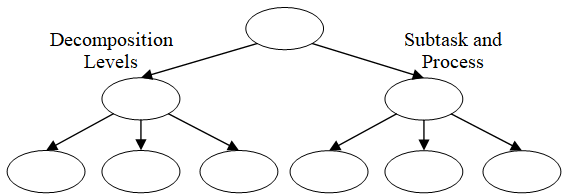
\includegraphics[width=1.0\linewidth]{fig1.png}
%\caption{Schematic representation of the computational domain, with the geometry parameterization points marked in red and the black points independent of the optimization iterations. The grey lines show the possible deformation of the geometry.}
%\label{fig}
%\end{figure}

The calculation was carried out ...

% Acknowledgement
\section{ACKNOWLEDGMENTS}
This study was supported by the Russian Science Foundation, project No 21-11-00204.



% References

%\nocite{*}
\bibliographystyle{aipnum-cp}%
\bibliography{bibliography}%


\end{document}
